\documentclass[border=15pt, multi, tikz]{standalone}
\usepackage{import}
\subimport{../../layers/}{init}
\usetikzlibrary{positioning}
\usetikzlibrary{3d} %for including external image 

\def\ConvColor{rgb:blue,5;green,2.5;white,5}
\def\ConvReluColor{rgb:yellow,5;red,5;white,5}
\def\PoolColor{rgb:red,1;black,0.3}
\def\DcnvColor{rgb:blue,5;green,2.5;white,5}
\def\SoftmaxColor{rgb:magenta,5;black,7}
\def\SumColor{rgb:blue,5;green,15}
\def\FcColor{rgb:blue,2;green,5;white,5}

\begin{document}
\begin{tikzpicture}
\tikzstyle{connection}=[ultra thick,every node/.style={sloped,allow upside down},draw=\edgecolor,opacity=0.7]
%%%%%%%%%%%%%%%%%%%%%%%%%%%%%%%%%%%%%%%%%%%%%%%%%%%%%%%%%%%%%%%%%%%%%%%%%%%%%%%%%%%%%%%%
%% Draw Layer Blocks
%%%%%%%%%%%%%%%%%%%%%%%%%%%%%%%%%%%%%%%%%%%%%%%%%%%%%%%%%%%%%%%%%%%%%%%%%%%%%%%%%%%%%%%%
\node[canvas is zy plane at x=0] (in) at (-7.9,0,0) {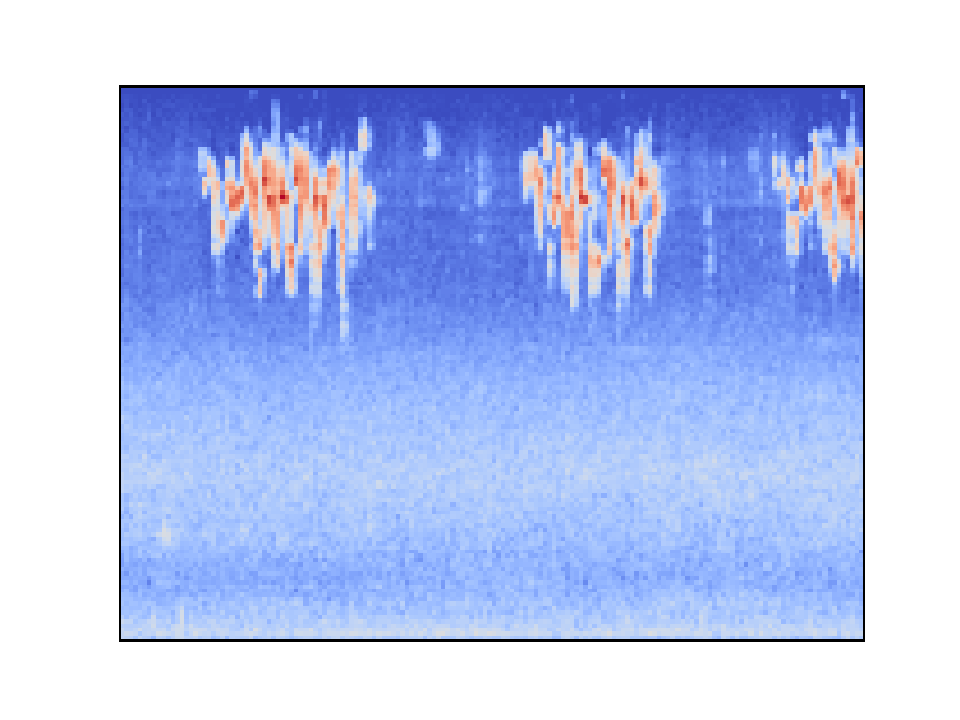
\includegraphics[width=8cm,height=8cm]{input.pdf}};
\node[canvas is zy plane at x=0] (norm) at (-5.2,0,0) {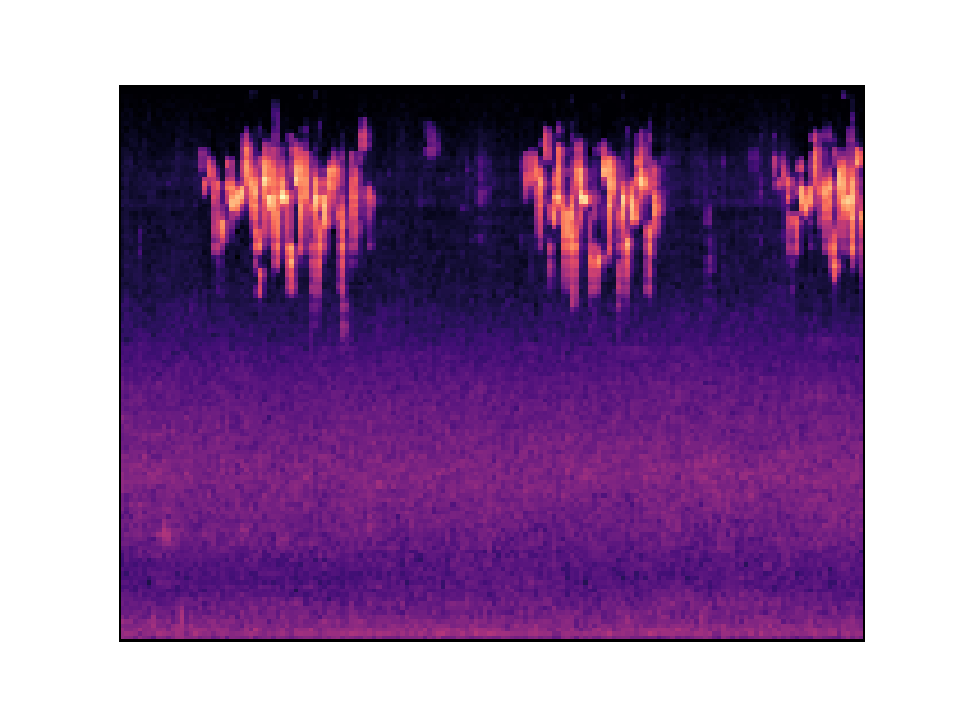
\includegraphics[width=8cm,height=8cm]{input_norm.pdf}};
\node[canvas is zy plane at x=0] (tfm) at (-2.5,0,0) {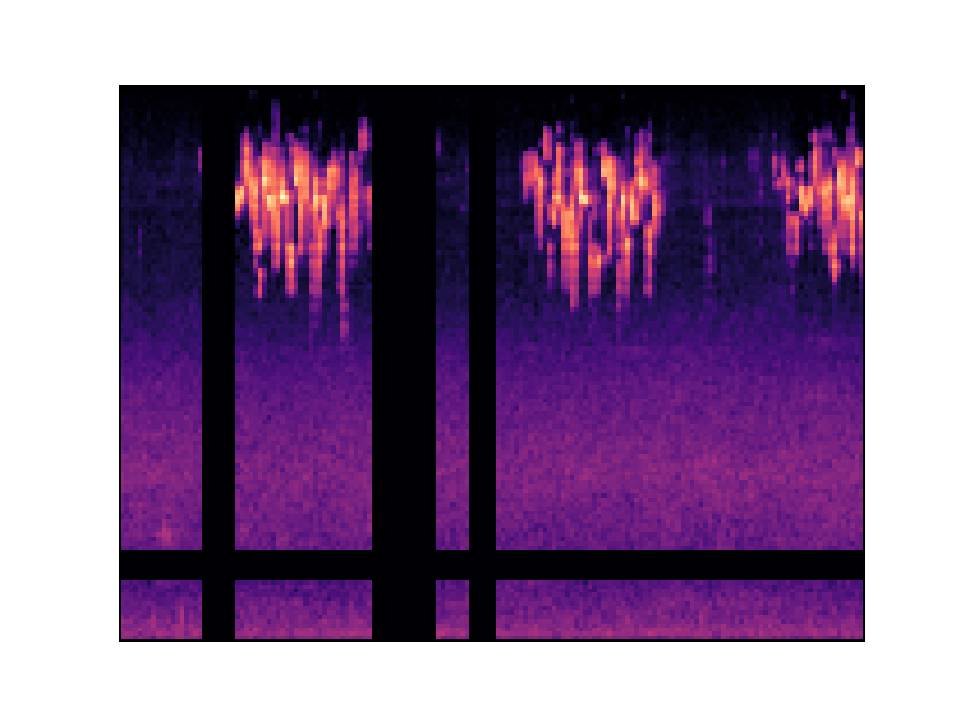
\includegraphics[width=8cm,height=8cm]{input_tfm.pdf}};

% Add captions below the images
\node[below=0.5cm of in, align=center] {\textbf{Input}};
\node[below=0.5cm of norm, align=center] {\textbf{Norm layer}};
\node[below=0.5cm of tfm, align=center] {\textbf{tfm layer}};

% conv1_1,conv1_2,%pool1
\pic[shift={(0.5,0,0)}] at (0,0,0) {Box={name=c1,caption=Conv~1 \\ {\(\mathbf{n = 64}\)},%
        fill=\ConvColor,%
        height=40,width={2},depth=40}};
% conv2_1,conv2_2,pool2
\pic[shift={(3.1,0,0)}] at (c1-east) {Box={name=c2,caption=Conv~2 \\ {\(\mathbf{n = 128}\)},%
        fill=\ConvColor,%
        height=30,width={7},depth=30}};

% conv3_1,conv3_2,pool3
\pic[shift={(2.4,0,0)}] at (c2-east) {Box={name=c3,caption=Conv~3 \\ {\(\mathbf{n = 128}\)},%
        fill=\ConvColor,%
        height=20,width={7},depth=20}};

\node[above, align=center, font=\Large\bfseries] at (11.2,0.15,0) {Flatten};

\pic[shift={(3.5,0,0)}] at (c3-east) 
{Box={
    name=d1,
    caption=Dense~1 \\ {\(\mathbf{n = 128}\)},
    fill=\FcColor,
    height=1.5,
    width=1.5,
    depth=40
    }
};

\pic[shift={(1.3,0,0)}] at (d1-east) 
{Box={
    name=d2,
    caption=Dense~2 \\ {\(\mathbf{n = 64}\)},
    fill=\FcColor,
    height=1.5,
    width=1.5,
    depth=20
    }
};

\pic[shift={(1.3,0,0)}] at (d2-east) 
{Box={
    name=out,
    caption=Out \\ {\(\mathbf{n = 46}\)},
    fill=\FcColor,
    height=1.5,
    width=1.5,
    depth=10
    }
};

%%%%%%%%%%%%%%%%%%%%%%%%%%%%%%%%%%%%%%%%%%%%%%%%%%%%%%%%%%%%%%%%%%%%%%%%%%%%%%%%%%%%%%%%
%% Draw connections
%%%%%%%%%%%%%%%%%%%%%%%%%%%%%%%%%%%%%%%%%%%%%%%%%%%%%%%%%%%%%%%%%%%%%%%%%%%%%%%%%%%%%%%%
\draw [connection] (-7.9,0,0) -- node {\midarrow} (-5.2,0,0); % from in to norm
\draw [connection] (-5.2,0,0) -- node {\midarrow} (-2.5,0,0);
\draw [connection] (-2.5,0,0) -- node {\midarrow} (c1-west);
\draw [connection]  (c1-east)    -- node {\midarrow} (c2-west);
\draw [connection]  (c2-east)    -- node {\midarrow} (c3-west);
\draw [connection]  (c3-east)    -- node {\midarrow} (d1-west); % [midway, above] {\huge\textcolor{black}{\textbf{Flatten}}}
\draw [connection]  (d1-east)    -- node {\midarrow} (d2-west);
\draw [connection]  (d2-east)    -- node {\midarrow} (out-west);
%%%%%%%%%%%%%%%%%%%%%%%%%%%%%%%%%%%%%%%%%%%%%%%%%%%%%%%%%%%%%%%%%%%%%%%%%%%%%%%%%%%%%%%%

\end{tikzpicture}
\end{document}\grid
